% Minimal LaTeX example for mediatr TikZ diagrams
% For articles/papers
\documentclass[12pt]{article}

% === Required for mediatr diagrams ===
\usepackage{tikz}
\usetikzlibrary{arrows.meta}
\usepackage{xcolor}

% === Optional but recommended ===
\usepackage[margin=1in]{geometry}

\begin{document}

\section*{Mediation Analysis}

% Option 1: Input from external file generated by mediatr
% In R: writeLines(tikz_code, "my_diagram.tex")
% \input{my_diagram.tex}

% Option 2: Inline example (what mediatr generates)
\begin{figure}[htbp]
\centering
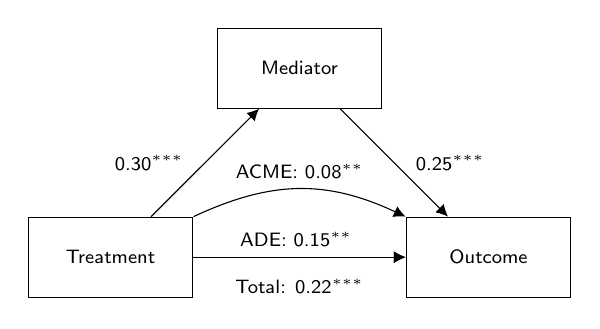
\begin{tikzpicture}[scale=0.4, >=stealth, font=\sffamily]
\scriptsize
\tikzset{mynode/.style={draw, text centered, text width = .75in, minimum height = .4in, align=center} }
\tikzset{>={Latex[width=1.5mm,length=1.5mm]}}
\node[mynode] (x) at (0,0)  {Treatment};
\node[mynode] (y) at (12,0) {Outcome};
\node[mynode] (m) at (6,6)  {Mediator};
\path[->] (x) edge node[above, align=center, yshift=1pt] {ADE: 0.15$^{**}$ } (y);
\path[->] (x) edge node[left, align=center, xshift=-5pt] {0.30$^{***}$} (m);
\path[->] (m) edge node[right, align=center, xshift=5pt] {0.25$^{***}$} (y);
\path[->] (x) edge node[below, align=center, yshift=-5pt] {Total: 0.22$^{***}$} (y);
\draw[->] (x.north east) to[out=25, in=155, looseness=1.05] node[midway, above, align=center, yshift=1pt] {ACME: 0.08$^{**}$} (y.north west);
\end{tikzpicture}
\caption{Example mediation diagram generated by \texttt{mediatr::med\_diagram\_acme\_tikz()}}
\end{figure}

\end{document}
